% Options for packages loaded elsewhere
\PassOptionsToPackage{unicode}{hyperref}
\PassOptionsToPackage{hyphens}{url}
%
\documentclass[
]{article}
\usepackage{lmodern}
\usepackage{amssymb,amsmath}
\usepackage{ifxetex,ifluatex}
\ifnum 0\ifxetex 1\fi\ifluatex 1\fi=0 % if pdftex
  \usepackage[T1]{fontenc}
  \usepackage[utf8]{inputenc}
  \usepackage{textcomp} % provide euro and other symbols
\else % if luatex or xetex
  \usepackage{unicode-math}
  \defaultfontfeatures{Scale=MatchLowercase}
  \defaultfontfeatures[\rmfamily]{Ligatures=TeX,Scale=1}
\fi
% Use upquote if available, for straight quotes in verbatim environments
\IfFileExists{upquote.sty}{\usepackage{upquote}}{}
\IfFileExists{microtype.sty}{% use microtype if available
  \usepackage[]{microtype}
  \UseMicrotypeSet[protrusion]{basicmath} % disable protrusion for tt fonts
}{}
\makeatletter
\@ifundefined{KOMAClassName}{% if non-KOMA class
  \IfFileExists{parskip.sty}{%
    \usepackage{parskip}
  }{% else
    \setlength{\parindent}{0pt}
    \setlength{\parskip}{6pt plus 2pt minus 1pt}}
}{% if KOMA class
  \KOMAoptions{parskip=half}}
\makeatother
\usepackage{xcolor}
\IfFileExists{xurl.sty}{\usepackage{xurl}}{} % add URL line breaks if available
\IfFileExists{bookmark.sty}{\usepackage{bookmark}}{\usepackage{hyperref}}
\hypersetup{
  pdftitle={Non additive interation},
  pdfauthor={Ziang Zhang},
  hidelinks,
  pdfcreator={LaTeX via pandoc}}
\urlstyle{same} % disable monospaced font for URLs
\usepackage[margin=1in]{geometry}
\usepackage{color}
\usepackage{fancyvrb}
\newcommand{\VerbBar}{|}
\newcommand{\VERB}{\Verb[commandchars=\\\{\}]}
\DefineVerbatimEnvironment{Highlighting}{Verbatim}{commandchars=\\\{\}}
% Add ',fontsize=\small' for more characters per line
\usepackage{framed}
\definecolor{shadecolor}{RGB}{248,248,248}
\newenvironment{Shaded}{\begin{snugshade}}{\end{snugshade}}
\newcommand{\AlertTok}[1]{\textcolor[rgb]{0.94,0.16,0.16}{#1}}
\newcommand{\AnnotationTok}[1]{\textcolor[rgb]{0.56,0.35,0.01}{\textbf{\textit{#1}}}}
\newcommand{\AttributeTok}[1]{\textcolor[rgb]{0.77,0.63,0.00}{#1}}
\newcommand{\BaseNTok}[1]{\textcolor[rgb]{0.00,0.00,0.81}{#1}}
\newcommand{\BuiltInTok}[1]{#1}
\newcommand{\CharTok}[1]{\textcolor[rgb]{0.31,0.60,0.02}{#1}}
\newcommand{\CommentTok}[1]{\textcolor[rgb]{0.56,0.35,0.01}{\textit{#1}}}
\newcommand{\CommentVarTok}[1]{\textcolor[rgb]{0.56,0.35,0.01}{\textbf{\textit{#1}}}}
\newcommand{\ConstantTok}[1]{\textcolor[rgb]{0.00,0.00,0.00}{#1}}
\newcommand{\ControlFlowTok}[1]{\textcolor[rgb]{0.13,0.29,0.53}{\textbf{#1}}}
\newcommand{\DataTypeTok}[1]{\textcolor[rgb]{0.13,0.29,0.53}{#1}}
\newcommand{\DecValTok}[1]{\textcolor[rgb]{0.00,0.00,0.81}{#1}}
\newcommand{\DocumentationTok}[1]{\textcolor[rgb]{0.56,0.35,0.01}{\textbf{\textit{#1}}}}
\newcommand{\ErrorTok}[1]{\textcolor[rgb]{0.64,0.00,0.00}{\textbf{#1}}}
\newcommand{\ExtensionTok}[1]{#1}
\newcommand{\FloatTok}[1]{\textcolor[rgb]{0.00,0.00,0.81}{#1}}
\newcommand{\FunctionTok}[1]{\textcolor[rgb]{0.00,0.00,0.00}{#1}}
\newcommand{\ImportTok}[1]{#1}
\newcommand{\InformationTok}[1]{\textcolor[rgb]{0.56,0.35,0.01}{\textbf{\textit{#1}}}}
\newcommand{\KeywordTok}[1]{\textcolor[rgb]{0.13,0.29,0.53}{\textbf{#1}}}
\newcommand{\NormalTok}[1]{#1}
\newcommand{\OperatorTok}[1]{\textcolor[rgb]{0.81,0.36,0.00}{\textbf{#1}}}
\newcommand{\OtherTok}[1]{\textcolor[rgb]{0.56,0.35,0.01}{#1}}
\newcommand{\PreprocessorTok}[1]{\textcolor[rgb]{0.56,0.35,0.01}{\textit{#1}}}
\newcommand{\RegionMarkerTok}[1]{#1}
\newcommand{\SpecialCharTok}[1]{\textcolor[rgb]{0.00,0.00,0.00}{#1}}
\newcommand{\SpecialStringTok}[1]{\textcolor[rgb]{0.31,0.60,0.02}{#1}}
\newcommand{\StringTok}[1]{\textcolor[rgb]{0.31,0.60,0.02}{#1}}
\newcommand{\VariableTok}[1]{\textcolor[rgb]{0.00,0.00,0.00}{#1}}
\newcommand{\VerbatimStringTok}[1]{\textcolor[rgb]{0.31,0.60,0.02}{#1}}
\newcommand{\WarningTok}[1]{\textcolor[rgb]{0.56,0.35,0.01}{\textbf{\textit{#1}}}}
\usepackage{graphicx,grffile}
\makeatletter
\def\maxwidth{\ifdim\Gin@nat@width>\linewidth\linewidth\else\Gin@nat@width\fi}
\def\maxheight{\ifdim\Gin@nat@height>\textheight\textheight\else\Gin@nat@height\fi}
\makeatother
% Scale images if necessary, so that they will not overflow the page
% margins by default, and it is still possible to overwrite the defaults
% using explicit options in \includegraphics[width, height, ...]{}
\setkeys{Gin}{width=\maxwidth,height=\maxheight,keepaspectratio}
% Set default figure placement to htbp
\makeatletter
\def\fps@figure{htbp}
\makeatother
\setlength{\emergencystretch}{3em} % prevent overfull lines
\providecommand{\tightlist}{%
  \setlength{\itemsep}{0pt}\setlength{\parskip}{0pt}}
\setcounter{secnumdepth}{5}

\title{Non additive interation}
\author{Ziang Zhang}
\date{3/25/2021}

\begin{document}
\maketitle

{
\setcounter{tocdepth}{2}
\tableofcontents
}
\hypertarget{the-underlying-model}{%
\section{The Underlying Model:}\label{the-underlying-model}}

In the first simulation study, we consider the following additive probit
model with non additive interaction:
\[Y^* = \beta_0+\beta_GG + \beta_EE + \gamma_1I(G=1)*E+\gamma_2I(G=2)*E + \epsilon\]
where \(\epsilon\sim N(0,\sigma^2)\) for some \textbf{known}
\(\sigma^2\).

This model is more general than the model with additive interaction
effect. When the interaction effect between \(G\) and \(E\) is actually
additive, we should have \(2\gamma_1 = \gamma_2\). Here our main
interest will be testing the null hypothesis \[H_0:\gamma_1=\gamma_2=0\]
without the information of \(E\).

Similar to the previous situation, the presence of term
\(\gamma_1,\gamma_2\) breaks the homoskedasiticiy assumption on
\(Var(Y^*|G)\), and hence result in a genotypic probit model (instead of
the additive model)
\[Y^* = \tilde{\gamma_0}+ \tilde{\gamma_1}I(G=1)+\tilde{\gamma_2}I(G=2)+ \tilde{\epsilon}\]
We will utilize the non-linearity test to test
\(H_0:2\tilde{\gamma_1}= \tilde{\gamma_2}\).

\hypertarget{simulation}{%
\section{Simulation :}\label{simulation}}

\hypertarget{an-example-when-the-interaction-effect-is-additive}{%
\subsection{An example when the interaction effect is
additive:}\label{an-example-when-the-interaction-effect-is-additive}}

\begin{Shaded}
\begin{Highlighting}[]
\CommentTok{### Read in data:}
\NormalTok{path <-}\StringTok{ "D:/gwas-practice/indep_QC.bed"}
\NormalTok{tmpfile  <-}\StringTok{ }\KeywordTok{tempfile}\NormalTok{()}
\KeywordTok{snp_readBed}\NormalTok{(path, }\DataTypeTok{backingfile =}\NormalTok{ tmpfile)}
\end{Highlighting}
\end{Shaded}

\begin{verbatim}
## [1] "C:\\Users\\aguer\\AppData\\Local\\Temp\\RtmpELe8GK\\file3b042503552b.rds"
\end{verbatim}

\begin{Shaded}
\begin{Highlighting}[]
\NormalTok{obj.bigSNP <-}\StringTok{ }\KeywordTok{snp_attach}\NormalTok{(}\KeywordTok{paste0}\NormalTok{(tmpfile , }\StringTok{".rds"}\NormalTok{))}

\NormalTok{G   <-}\StringTok{ }\NormalTok{obj.bigSNP}\OperatorTok{$}\NormalTok{genotypes}
\NormalTok{CHR <-}\StringTok{ }\NormalTok{obj.bigSNP}\OperatorTok{$}\NormalTok{map}\OperatorTok{$}\NormalTok{chromosome}
\NormalTok{POS <-}\StringTok{ }\NormalTok{obj.bigSNP}\OperatorTok{$}\NormalTok{map}\OperatorTok{$}\NormalTok{physical.pos}

\CommentTok{### Randomly Sample p genes}
\KeywordTok{set.seed}\NormalTok{(}\DecValTok{123}\NormalTok{,}\DataTypeTok{sample.kind=}\StringTok{"Rounding"}\NormalTok{)}
\NormalTok{p <-}\StringTok{ }\DecValTok{5}
\CommentTok{### Need to make sure that all genotypes have enough frequencies in the selected genes:}
\NormalTok{freq_counts <-}\StringTok{ }\KeywordTok{big_counts}\NormalTok{(G)}
\NormalTok{MAF <-}\StringTok{ }\KeywordTok{snp_MAF}\NormalTok{(G)}
\NormalTok{Qualified <-}\StringTok{ }\NormalTok{freq_counts[}\DecValTok{3}\NormalTok{,] }\OperatorTok{>=}\StringTok{ }\DecValTok{200} \OperatorTok{&}\StringTok{ }\NormalTok{MAF}\OperatorTok{>=}\FloatTok{0.3}
\NormalTok{indx <-}\StringTok{ }\KeywordTok{which}\NormalTok{(POS }\OperatorTok\StringTok{ }\KeywordTok{sample}\NormalTok{(POS[Qualified], }\DataTypeTok{size =}\NormalTok{ p))}
\NormalTok{G_use <-}\StringTok{ }\NormalTok{G[,indx]}
\NormalTok{POS_use <-}\StringTok{ }\NormalTok{POS[indx]}
\NormalTok{CHR_use <-}\StringTok{ }\NormalTok{CHR[indx]}
\CommentTok{### Do the bootstrapping:}
\NormalTok{bootsize <-}\StringTok{ }\DecValTok{5000}
\NormalTok{G_boot <-}\StringTok{ }\NormalTok{G_use[}\KeywordTok{sample}\NormalTok{(}\DecValTok{1}\OperatorTok{:}\KeywordTok{nrow}\NormalTok{(G_use), bootsize, }\DataTypeTok{replace=}\OtherTok{TRUE}\NormalTok{), ]}

\CommentTok{### Specify a set of parameter, Compute power:}
\NormalTok{b0 <-}\StringTok{ }\DecValTok{-1}
\NormalTok{bG <-}\StringTok{ }\FloatTok{0.3}
\NormalTok{gam1 <-}\StringTok{ }\FloatTok{0.3}
\NormalTok{gam2 <-}\StringTok{ }\FloatTok{0.6}
\NormalTok{bE <-}\StringTok{ }\FloatTok{0.3}
\NormalTok{sig <-}\StringTok{ }\DecValTok{1}
\NormalTok{sigmaE <-}\StringTok{ }\DecValTok{1}
\NormalTok{measure_error_percentage <-}\StringTok{ }\DecValTok{1}\OperatorTok{/}\DecValTok{4}
\NormalTok{power <-}\StringTok{ }\KeywordTok{Interaction_Test}\NormalTok{(}\DataTypeTok{G =}\NormalTok{ G_boot[,}\DecValTok{1}\NormalTok{], b0, bG, gam1, gam2, bE, sig, sigmaE, }\DataTypeTok{K =} \DecValTok{10000}\NormalTok{, }\DataTypeTok{measure_error_percentage =} \DecValTok{1}\OperatorTok{/}\DecValTok{4}\NormalTok{)}
\KeywordTok{apply}\NormalTok{(}\KeywordTok{as.matrix}\NormalTok{(power)}\OperatorTok{<=}\FloatTok{0.05}\NormalTok{, }\DecValTok{2}\NormalTok{, mean)}
\end{Highlighting}
\end{Shaded}

\begin{verbatim}
##  proposed     withE withError 
##     0.099     1.000     1.000
\end{verbatim}

\begin{Shaded}
\begin{Highlighting}[]
\NormalTok{power }\OperatorTok\StringTok{ }\KeywordTok{pivot_longer}\NormalTok{(proposed}\OperatorTok{:}\NormalTok{withError, }\DataTypeTok{values_to =} \StringTok{"P"}\NormalTok{, }\DataTypeTok{names_to =} \StringTok{"type"}\NormalTok{) }\OperatorTok\StringTok{ }\KeywordTok{ggplot}\NormalTok{(}\KeywordTok{aes}\NormalTok{(P)) }\OperatorTok{+}\StringTok{ }\KeywordTok{geom_histogram}\NormalTok{(}\DataTypeTok{bins =} \DecValTok{20}\NormalTok{) }\OperatorTok{+}\StringTok{ }\KeywordTok{facet_grid}\NormalTok{(}\OperatorTok{~}\NormalTok{type)}
\end{Highlighting}
\end{Shaded}

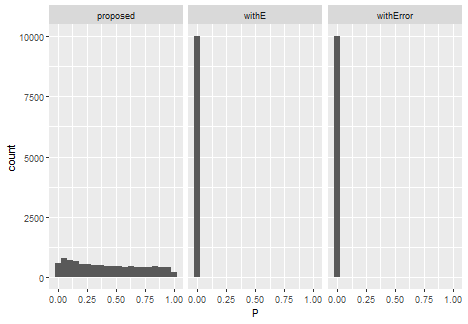
\includegraphics{simulation_bootstrapping_files/figure-latex/unnamed-chunk-2-1.png}

\hypertarget{an-example-when-the-interaction-effect-is-non-additive}{%
\subsection{An example when the interaction effect is
non-additive:}\label{an-example-when-the-interaction-effect-is-non-additive}}

\begin{Shaded}
\begin{Highlighting}[]
\CommentTok{### Randomly Sample p genes}
\KeywordTok{set.seed}\NormalTok{(}\DecValTok{123}\NormalTok{,}\DataTypeTok{sample.kind=}\StringTok{"Rounding"}\NormalTok{)}
\NormalTok{p <-}\StringTok{ }\DecValTok{5}
\CommentTok{### Need to make sure that all genotypes have enough frequencies in the selected genes:}
\NormalTok{freq_counts <-}\StringTok{ }\KeywordTok{big_counts}\NormalTok{(G)}
\NormalTok{MAF <-}\StringTok{ }\KeywordTok{snp_MAF}\NormalTok{(G)}
\NormalTok{Qualified <-}\StringTok{ }\NormalTok{freq_counts[}\DecValTok{3}\NormalTok{,] }\OperatorTok{>=}\StringTok{ }\DecValTok{200} \OperatorTok{&}\StringTok{ }\NormalTok{MAF}\OperatorTok{>=}\FloatTok{0.3}
\NormalTok{indx <-}\StringTok{ }\KeywordTok{which}\NormalTok{(POS }\OperatorTok\StringTok{ }\KeywordTok{sample}\NormalTok{(POS[Qualified], }\DataTypeTok{size =}\NormalTok{ p))}
\NormalTok{G_use <-}\StringTok{ }\NormalTok{G[,indx]}
\NormalTok{POS_use <-}\StringTok{ }\NormalTok{POS[indx]}
\NormalTok{CHR_use <-}\StringTok{ }\NormalTok{CHR[indx]}
\CommentTok{### Do the bootstrapping:}
\NormalTok{bootsize <-}\StringTok{ }\DecValTok{5000}
\NormalTok{G_boot <-}\StringTok{ }\NormalTok{G_use[}\KeywordTok{sample}\NormalTok{(}\DecValTok{1}\OperatorTok{:}\KeywordTok{nrow}\NormalTok{(G_use), bootsize, }\DataTypeTok{replace=}\OtherTok{TRUE}\NormalTok{), ]}

\CommentTok{### Specify a set of parameter, Compute power:}
\NormalTok{b0 <-}\StringTok{ }\DecValTok{-1}
\NormalTok{bG <-}\StringTok{ }\FloatTok{0.3}
\NormalTok{gam1 <-}\StringTok{ }\FloatTok{0.3}
\NormalTok{gam2 <-}\StringTok{ }\DecValTok{0}
\NormalTok{bE <-}\StringTok{ }\FloatTok{0.3}
\NormalTok{sig <-}\StringTok{ }\DecValTok{1}
\NormalTok{sigmaE <-}\StringTok{ }\DecValTok{1}
\NormalTok{measure_error_percentage <-}\StringTok{ }\DecValTok{1}\OperatorTok{/}\DecValTok{4}
\NormalTok{power <-}\StringTok{ }\KeywordTok{Interaction_Test}\NormalTok{(}\DataTypeTok{G =}\NormalTok{ G_boot[,}\DecValTok{1}\NormalTok{], b0, bG, gam1, gam2, bE, sig, sigmaE, }\DataTypeTok{K =} \DecValTok{10000}\NormalTok{, }\DataTypeTok{measure_error_percentage =} \DecValTok{1}\OperatorTok{/}\DecValTok{4}\NormalTok{)}
\KeywordTok{apply}\NormalTok{(}\KeywordTok{as.matrix}\NormalTok{(power)}\OperatorTok{<=}\FloatTok{0.05}\NormalTok{, }\DecValTok{2}\NormalTok{, mean)}
\end{Highlighting}
\end{Shaded}

\begin{verbatim}
##  proposed     withE withError 
##    0.3978    0.4315    0.3536
\end{verbatim}

\begin{Shaded}
\begin{Highlighting}[]
\NormalTok{power }\OperatorTok\StringTok{ }\KeywordTok{pivot_longer}\NormalTok{(proposed}\OperatorTok{:}\NormalTok{withError, }\DataTypeTok{values_to =} \StringTok{"P"}\NormalTok{, }\DataTypeTok{names_to =} \StringTok{"type"}\NormalTok{) }\OperatorTok\StringTok{ }\KeywordTok{ggplot}\NormalTok{(}\KeywordTok{aes}\NormalTok{(P)) }\OperatorTok{+}\StringTok{ }\KeywordTok{geom_histogram}\NormalTok{(}\DataTypeTok{bins =} \DecValTok{20}\NormalTok{) }\OperatorTok{+}\StringTok{ }\KeywordTok{facet_grid}\NormalTok{(}\OperatorTok{~}\NormalTok{type)}
\end{Highlighting}
\end{Shaded}

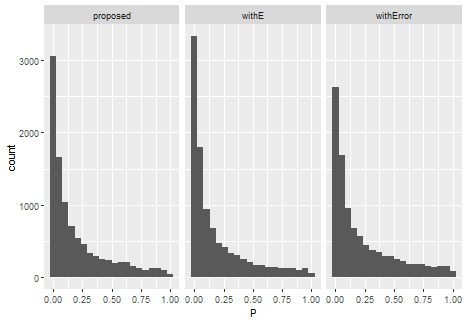
\includegraphics{simulation_bootstrapping_files/figure-latex/unnamed-chunk-3-1.png}

\hypertarget{study-of-type-i-error-rate}{%
\subsection{Study of Type I error
rate:}\label{study-of-type-i-error-rate}}

\begin{Shaded}
\begin{Highlighting}[]
\KeywordTok{set.seed}\NormalTok{(}\DecValTok{123}\NormalTok{,}\DataTypeTok{sample.kind=}\StringTok{"Rounding"}\NormalTok{)}
\NormalTok{bootsize <-}\StringTok{ }\DecValTok{5000}
\NormalTok{G_boot <-}\StringTok{ }\NormalTok{G_use[}\KeywordTok{sample}\NormalTok{(}\DecValTok{1}\OperatorTok{:}\KeywordTok{nrow}\NormalTok{(G_use), bootsize, }\DataTypeTok{replace=}\OtherTok{TRUE}\NormalTok{), ]}

\CommentTok{### Specify a set of parameter, compute Type I error rate}
\NormalTok{b0 <-}\StringTok{ }\DecValTok{-1}
\NormalTok{bG <-}\StringTok{ }\FloatTok{0.3}
\NormalTok{gam1 <-}\StringTok{ }\DecValTok{0}
\NormalTok{gam2 <-}\StringTok{ }\DecValTok{0}
\NormalTok{bE <-}\StringTok{ }\FloatTok{0.3}
\NormalTok{sig <-}\StringTok{ }\DecValTok{1}
\NormalTok{sigmaE <-}\StringTok{ }\DecValTok{1}
\NormalTok{measure_error_percentage <-}\StringTok{ }\DecValTok{1}\OperatorTok{/}\DecValTok{4}
\NormalTok{error <-}\StringTok{ }\KeywordTok{Interaction_Test}\NormalTok{(}\DataTypeTok{G =}\NormalTok{ G_boot[,}\DecValTok{1}\NormalTok{], b0, bG, gam1, gam2, bE, sig, sigmaE, }\DataTypeTok{K =} \DecValTok{10000}\NormalTok{, }\DataTypeTok{measure_error_percentage =} \DecValTok{1}\OperatorTok{/}\DecValTok{4}\NormalTok{)}
\KeywordTok{apply}\NormalTok{(}\KeywordTok{as.matrix}\NormalTok{(error)}\OperatorTok{<=}\FloatTok{0.05}\NormalTok{, }\DecValTok{2}\NormalTok{, mean)}
\end{Highlighting}
\end{Shaded}

\begin{verbatim}
##  proposed     withE withError 
##    0.0493    0.0483    0.0504
\end{verbatim}

\begin{Shaded}
\begin{Highlighting}[]
\NormalTok{error }\OperatorTok\StringTok{ }\KeywordTok{pivot_longer}\NormalTok{(proposed}\OperatorTok{:}\NormalTok{withError, }\DataTypeTok{values_to =} \StringTok{"P"}\NormalTok{, }\DataTypeTok{names_to =} \StringTok{"type"}\NormalTok{) }\OperatorTok\StringTok{ }\KeywordTok{ggplot}\NormalTok{(}\KeywordTok{aes}\NormalTok{(P)) }\OperatorTok{+}\StringTok{ }\KeywordTok{geom_histogram}\NormalTok{(}\DataTypeTok{bins =} \DecValTok{30}\NormalTok{) }\OperatorTok{+}\StringTok{ }\KeywordTok{facet_grid}\NormalTok{(}\OperatorTok{~}\NormalTok{type) }\OperatorTok{+}\StringTok{ }\KeywordTok{xlim}\NormalTok{(}\DecValTok{0}\NormalTok{,}\DecValTok{1}\NormalTok{)}
\end{Highlighting}
\end{Shaded}

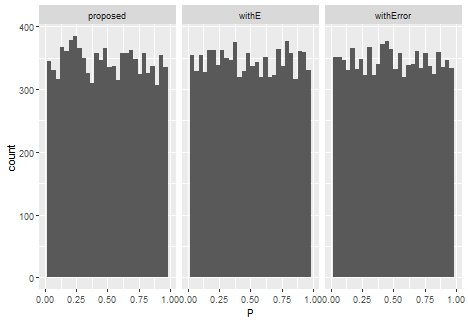
\includegraphics{simulation_bootstrapping_files/figure-latex/unnamed-chunk-4-1.png}

\end{document}
